\documentclass[a4paper, 12pt]{article}
% Allows writing the document in French.
\usepackage[T1]{fontenc}
\usepackage[utf8]{inputenc}
\usepackage[francais]{babel}
% Allows to change the margins of the pages.
\usepackage[margin=2.5cm]{geometry}
% Allows to change the line spacing.
\renewcommand{\baselinestretch}{1.5}
% Provides generic commands \degree, \celsius, etc.
\usepackage{gensymb}
% Allows to use images.
\usepackage{graphicx}
% Includes pseudocode or algorithms.
\usepackage{listings, lstautogobble}
% Allows change items properties
\usepackage{enumitem}
% Adds space between paragraphs.
\usepackage{parskip}
% Supports Text Companion fonts (necessary for gensymb).
\usepackage{textcomp}
% Allows to create better tables.
\usepackage{tabularx}
% Allows to draw.
\usepackage{tikz}
% Allows to color the raw of an array.
\usepackage{colortbl}
% Allows to use colors.
\usepackage{xcolor}
% Allows hyperlinks within the document.
\usepackage[colorlinks=true,urlcolor=black,linkcolor=black]{hyperref}
% Allows to use copyright.
\usepackage[
    type={CC},
    modifier={by-nc-nd},
    version={4.0},
    ]{doclicense}

% Allows a better depth for the table of contents.
\setcounter{tocdepth}{4}
% Allows a better depth for the sections.
\setcounter{secnumdepth}{4}

% New column type
\newcolumntype{L}{>{\raggedright\arraybackslash}X}
\newcolumntype{C}{>{\centering\arraybackslash}X}
\newcolumntype{R}{>{\raggedleft\arraybackslash}X}

% Define colors for color scheme
\definecolor{background}{HTML}{333333}
\definecolor{currentLine}{HTML}{282A2E}
\definecolor{selection}{HTML}{373B41}
\definecolor{foreground}{HTML}{FFFFFF}
\definecolor{comment}{HTML}{969896}
\definecolor{red}{HTML}{CC6666}
\definecolor{orange}{HTML}{DE935F}
\definecolor{yellow}{HTML}{F0C674}
\definecolor{green}{HTML}{B5BD68}
\definecolor{aqua}{HTML}{8ABEB7}
\definecolor{blue}{HTML}{81A2bE}
\definecolor{purple}{HTML}{B294BB}
\definecolor{bleuSkype}{HTML}{00AFF0}
\definecolor{jauneSnapchat}{HTML}{FFFC00}

% Macro
\makeatletter
\lst@InstallKeywords k{attributes}{attributestyle}\slshape{attributestyle}{}ld
\makeatother

% Custom color scheme for batch
\lstset{language=bash,
		numbers=left,
		numberstyle=\tiny,
		autogobble=true,
		backgroundcolor=\color{background},
		commentstyle=\color{comment},
		stringstyle=\color{green},
		keywordstyle=\color{red},
		keywords={home, root, user, @, \$},
		basicstyle=\ttfamily\color{foreground},
		attributestyle=\color{aqua},
		moreattributes={ls, now}
              }

              \lstset {
                literate={~} {$\sim$}{1}
              }

% Allows draw lines for the flyleaf.
\newcommand{\HRule}{\rule{\linewidth}{0.5mm}}

% Starts roman numbering (trick to not numbering the first pages).
\pagenumbering{roman}

\begin{document}
\renewcommand{\bibname}{Références}
\begin{center}
  
  \begin{figure}[!h]
    \centering
    
\includegraphics[width=0.25\textwidth]{textures/logo/heh_bw.eps}    
  \end{figure}

  \textsc{\LARGE Serveur Linux} \\ [0.5cm]
  \textsc{\Large Installation et configuration} \\ [0.5cm]

  \textsc{\large 2\up{ème} Bachelier en Informatique} \\ [0.2cm]

  \begingroup
  \fontfamily{pag} \selectfont 

  \HRule \\ [0.4cm] {
    \huge Projet Linux \\ [0.2cm] 
  }
  \HRule \\ [1.3cm]
  \endgroup

  \begin{minipage}[t]{0.4 \textwidth} 
    \begin{flushleft} 
      \large \emph{Auteur:} \\ 
      Terencio \textsc{Agozzino}
    \end{flushleft} 
  \end{minipage}
  % 
  \begin{minipage}[t]{0.4 \textwidth}
    \begin{flushright} 
      \large \emph{Auteur :} \\ 
      Alexandre \textsc{Ducobu}
    \end{flushright} 
  \end{minipage}

  \vspace{1.5cm}

  \begin{minipage}[t]{0.4 \textwidth}
    \begin{center} 
      \large \emph{Enseignants:} \\ 
      Antoine \textsc{Malaise} \\
      Julien \textsc{De Bodt}
    \end{center} 
  \end{minipage}

  \vspace{1cm}

  \begin{figure}[!h]
    \centering
    
\includegraphics[scale=0.08]{textures/logo/technical_bw.pdf}
  \end{figure}
  
  \vspace{0.5cm}

  Année académique 2016 - 2017
\end{center}

\thispagestyle{empty}

\newpage
\newpage
\thispagestyle{empty}
\setcounter{page}{0}
\null
\newpage
\begin{center}
  
\includegraphics[scale=0.12]{textures/logo/heh.pdf}

  \vspace{1cm}

  \textsc{\LARGE Serveur Linux} \\ [0.5cm]
  \textsc{\Large Installation et configuration} \\ [0.5cm]

  \textsc{\large 2\up{ème} Bachelier en Informatique} \\ [0.2cm]

  \begingroup
  \fontfamily{pag} \selectfont 

  \HRule \\ [0.4cm] {
    \huge Projet Linux \\ [0.2cm] 
  }
  \HRule \\ [1.3cm]
  \endgroup

  \begin{minipage}[t]{0.4 \textwidth} 
    \begin{flushleft} 
      \large \emph{Auteur:} \\ 
      Terencio \textsc{Agozzino}
    \end{flushleft} 
  \end{minipage}
  % 
  \begin{minipage}[t]{0.4 \textwidth}
    \begin{flushright} 
      \large \emph{Auteur :} \\ 
      Alexandre \textsc{Ducobu}
    \end{flushright} 
  \end{minipage}

  \vspace{1.5cm}

  \begin{minipage}[t]{0.4 \textwidth}
    \begin{center} 
      \large \emph{Enseignants:} \\ 
      Antoine \textsc{Malaise} \\
      Julien \textsc{De Bodt}
    \end{center} 
  \end{minipage}

  \vspace{1cm}

  
\includegraphics[scale=0.08]{textures/logo/technical.pdf}

  \vspace{0.5cm}

  Année académique 2016 - 2017
\end{center}

\thispagestyle{empty}

\newpage
\newpage
\thispagestyle{empty}
\setcounter{page}{0}
\null
\newpage
\newpage
\mbox{~}
\vfill
Ce document est mis à disposition selon les termes de la licence Creative
Commons “\href{https://creativecommons.org/licenses/by-nc-nd/4.0/}{Attribution
- Pas d'utilisation commerciale 4.0 International}”.

\begin{center}
  
\includegraphics[scale=1]
    {textures/images/license/license.pdf}
\end{center}
\setcounter{page}{0}
\thispagestyle{empty}

\newpage
\pagenumbering{arabic}
\tableofcontents
\newpage
\section{Présentation générale du projet}
\label{sec:pres-gener-du}


\subsection{Introduction}
\label{sec:introduction}

Dans le cadre de ce projet, il nous a été demandé d'administrer un serveur sous
Linux. \\
Le choix de la distribution ainsi que la gestion des sauvegardes est libre et
devra être justifié. \\

Le serveur devra contenir :

\begin{itemize}
    \item un partage \textbf{NFS} qui permettra aux utilisateurs du réseaux local d'y stocker des fichiers;
    \item un partage \textbf{Samba} permettra aux utilisateurs Windows d'accéder à ce même partage;
    \item un serveur \textbf{Web}, \textbf{FTP}, \textbf{MySQL} et \textbf{DNS} qui permettra un hébergement multi-utilisateurs;
    \begin{itemize}
        \item[$\bullet$] le FTP permettra à chaque utilisateur d'accéder à son dossier Web;
        \item[$\bullet$] il faudra créer une zone dans le DNS pour nos sites;
        \item[$\bullet$] le DNS fera également office de DNS cache pour le réseau local;
    \end{itemize}
    \item un \textbf{serveur de temps} pour que les machines du
    réseau local puissent se synchroniser;
    \item une connexion en \textbf{SSH} au serveur.
\end{itemize}


\newpage


\subsection{Déontologie}
\label{sec:déontologie}

En tant qu'administrateurs du serveur, nous serons tenus de suivre de nombreuses
règles telles que :

\begin{itemize}
    \item la documentation des actions entreprises sur le serveur;
    \item l'automatisation des installations et configurations au travers de scripts;
    \item la sécurité : mise en place de mots de passe forts, du SSH, etc.
    \item la vigilance et la prévoyance, par exemple par la mise en place de
    sauvegardes avant et après chaque changements sur le serveur;
    \item le contrôle du bon fonctionnement de chaque élément.
\end{itemize}


\subsection{Sécurité}
\label{sec:securite}

Du côté de la sécurité, nous avons quelques contraintes reprises ci-dessous :

\begin{itemize}
    \item mise en place d'une politique utilisateur;
    \item mise en place de quotas;
    \item partitionnement et gestion du disque \textit{(\textbf{LVM} et
    \textbf{RAID})};
    \item mise en place d'une stratégie de sauvegarde;
    \item désactivation des éléments inutiles et des mises à jours;
    \item mise en place d'un antivirus, d'un firewall, etc.
\end{itemize}

%%% Local Variables:
%%% mode: latex
%%% TeX-master: t
%%% End:

\newpage

\chapter*{Installation} %On garde ?
\label{cha:installation}

\section{Choix}
\label{sec:choix}

\subsection{Distribution}
\label{sec:distribution}

Notre choix de la distribution s'est naturellement porté sur Debian, pour ses
nombreux avantages. En voici quelques exemples :

\begin{itemize}
\item Large communauté : grâce à cela, les erreurs et problèmes rencontrés ont
  souvent plusieurs solutions connues et éprouvées.

\item Plusieurs architectures et noyaux : Debian supporte la majorité des
  architectures de processeurs comme AMD, Armel, i386, MIPS, etc. Elle supporte
  aussi de nombreux noyaux tels que FreeBSD et GNU Hurd.

\item Sécurité : vu que la distribution est open-source, cela signifie que les
  backdoors sont presque inexistantes. De surcroît, lorsqu'une faille de sécurité
  est détectée, celle-ci est rapidement corrigée par la communauté.

  En outre, Debian comprend de nombreux logiciels de sécurité tels que GPG (et
  PGP), SSH et autres.

\item Stabilité : nous savons que les serveurs doivent avoir le plus grand temps
d'accessibilité ($\approx$ 99.999\%). Sous Debian, il existe de nombreux exemples de
machines qui tournent sans arrêt pendant des années, mis à part lors de pannes
ou de mises à jour matérielles.

\item Système de paquets : grâce au système de paquets, les distributions Linux
ont la possibilité d'installer de nombreux logiciels par une seule ligne de
commande. Le système de paquets de Debian est l'outil central de mise à jour,
installation, suppression et recherche de paquets.
\end{itemize}

\newpage

De même, la distribution Debian est plus professionnel et celle-ci possède le
leadership depuis des années.

À titre d'information, depuis mai 2016, Ubuntu a les mêmes parts de marché que
Debian.

\begin{figure}[!h]
    \centering
    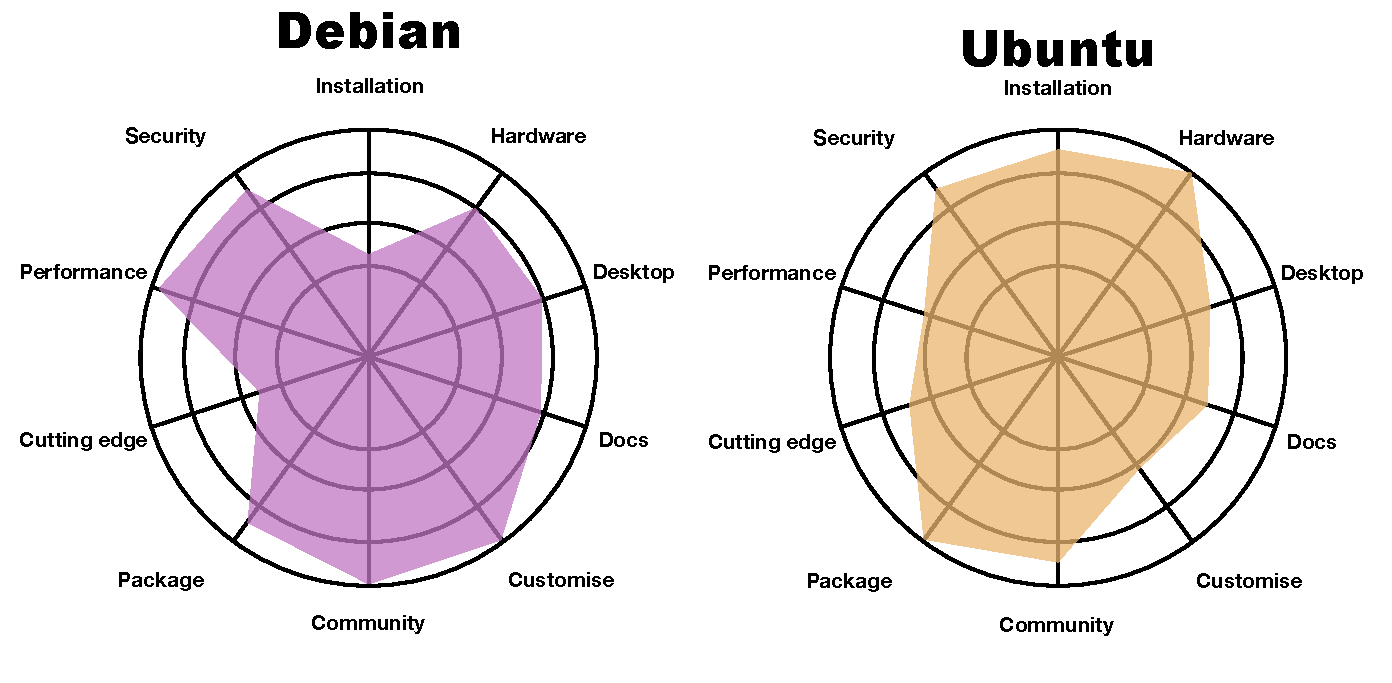
\includegraphics[scale=0.4]
    {textures/images/installation/DebianVsUbuntu.pdf}
    \caption{Différences entre Debian et Ubuntu}
     \label{fig:diff-debian-ubuntu}
  \end{figure}

Nous n'avons pas choisi Ubuntu pour les raisons suivantes :

\begin{itemize}
\item C'est un dérivé de Debian : de ce fait, un administrateur sachant
  configurer un serveur Debian pourra faciliter s'adapter au serveur Ubuntu.

\item Il vise le grand public et, de ce fait, est beaucoup moins utilisé
  dans le milieu professionnel.

\item Celui-ci est assez récent sur le marché du serveur.

\item Moins performant que Debian.
\end{itemize}

Concernant les autres distributions, CentOS est en baisse, mais reste au-dessus
de Red Hat et de Fedora qui, lui, est en chute libre.

\begin{figure}[h]
  \centering
  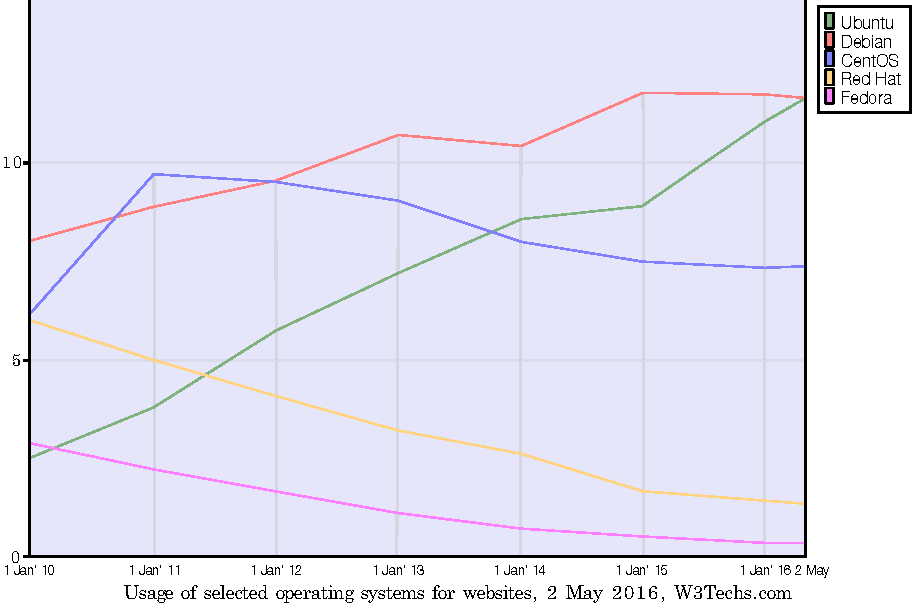
\includegraphics[scale=0.63]
  {textures/images/installation/distributions.pdf}
  \caption{Parts de marché des distributions Linux}
\end{figure}

\newpage

\subsection{Langue}
\label{sec:langue}

Pour le choix de la langue lors de l'installation, il a été préféré d'utiliser
l'anglais vu que la majorité des documentations et forums sont disponibles dans
cette langue. De plus, cela permet d'éviter une mauvaise traduction concernant
les nouvelles mises à jour et de toucher un plus large public possible.

\subsection{Noyau}
\label{sec:noyau}

Un noyau (monolithique) modulaire a été choisi afin de gérer les
modules. En effet, celui-ci facilite l'ajout et la suppression de modules à
chaud. Ces modules, pas toujours indispensables, peuvent être la source de
failles et de bugs.

\subsection{Partitionnement}
\label{sec:partitionnement}

Nous avons partitionné le disque de cette manière, avec un partition racine,
\textit{/boot}, et un groupe de volume LVM, \textit{VolGroup} : \\

\begin{center}
    \begin{table}[h]
        \begin{tabularx}{\linewidth}{|C|C|C|C|}
            \hline
            Label & Type & Taille (Mo) & Format \\
            \hline
            \hline
            /boot & primary & 512 & ext4 \\
            \hline
            VolGroup & logical & 20958 & lvm \\
            \hline
        \end{tabularx}

        \vskip .5cm

        \begin{tabularx}{\linewidth}{|C|C|C|C|}
            \hline
            LVsrv (/srv) & lvm & 6144 & ext4 \\
            %web et nfs
            \hline
            LVswap (/swap) & lvm & 4096 & swap \\
            \hline
            LVhome (/home) & lvm & 2048 & ext4 \\
            \hline
            LVroot (/root) & lvm & 2048 & ext4 \\
            \hline
            LVusr (/usr) & lvm & 2048 & ext4 \\
            \hline
            LVopt (/opt) & lvm & 2048 & ext4 \\
            \hline
            LVvar (/var) & lvm & 1024 & ext4 \\
            \hline
            LVtmp (/tmp) & lvm & 1024 & ext4 \\
            \hline
        \end{tabularx}
        \caption{Tableau du partitionnement \textit{(avec LVM)}}
        \label{tab:tableau-partitionnement}
    \end{table}
\end{center}

%%% Local Variables:
%%% mode: latex
%%% TeX-master: t
%%% End:

\newpage
\section{Services}
\label{sec:services}

\subsection{NTP}
\label{subsec:ntp}

Le \textbf{NTP}, ou \textit{\textbf{Network Time Protocol}}, est le protocole que nous
avons utilisé afin de synchroniser les machines du réseau local avec l'horloge
du serveur.


\subsubsection{Principe}
\label{subsubsec:principe}

En effet, bien que tout équipement informatique dispose d'une horloge, celle-ci
dérive comme toute montre ordinaire, ce qui peut amener des erreurs de
synchronisation. \\
La nécessité de synchroniser des équipements en réseau paraît alors évidente. \\

Chaque machine peut être à la fois serveur et client.\\
Elle sélectionnera un serveur de temps dans sa configuration, et récupérera
l'heure, ainsi qu'un numéro de strate, \textit{\textbf{n}}, et se déclarera
de strate \textit{\textbf{n+1}}.\\

L'architecture du réseau est en arborescence, et divisée en trois couches :
\begin{enumerate}

    \item les sources les plus précises \textit{(horloges atomiques,
    récepteurs GPS…)} sont de \textbf{strate 0};
    \item les serveurs diffusant l'heure des sources sont de \textbf{strate 1};
    \item les serveurs de \textbf{strate 2} sont généralement accessibles au public.

\end{enumerate}


\subsubsection{Configuration du serveur}
\label{subsubsec:configuration-serveur}

Voici les différentes étapes et options que nous avons effectuées :
\begin{itemize}

    \item[$\bullet$] activation des statistiques NTP;
    \item[$\bullet$] ajout de trois serveurs \textit{(un belge et deux européens)};
    \item[$\bullet$] activation de l'échange de l'heure avec tout le monde
    \textit{(aucune modification n'est acceptée)};
    \item[$\bullet$] activation de la synchronisation avec les machines du
    réseau local.

\end{itemize}


\subsubsection{Configuration du client}
\label{subsubsec:configuration-client}

Sur le client, la configuration est beaucoup plus simple :
\begin{itemize}

    \item[$\bullet$] activation des statistiques NTP;
    \item[$\bullet$] ajout du serveur local.

\end{itemize}


%%% Local Variables:
%%% mode: latex
%%% TeX-master: t
%%% End:

\newpage
\section{SSH}
\label{sec:ssh}

Le \textbf{SSH}, ou \textit{\textbf{Secure Shell}}, est un protocole de
communication sécurisé. Il impose un échange de clés de chiffrement en début de
connexion.


\subsection{Type d'authentification}
\label{subsec:type-authentification}

Il y a plusieurs façons de s'authentifier sur le serveur via SSH. \\
Les deux plus utilisées sont :
\begin{itemize}
    \item l'authentification par mot de passe;
    \item l'authentification par clés publique et privée du client. \\
\end{itemize}

Nous avons décidé de mettre en place une \textbf{identification automatique par
clés}. Ainsi on évite d'entrer le mot de passe à chaque connexion à distance. \\
Cette méthode est plus complexe à mettre en place, mais elle surtout plus
pratique. \\

On remarque rapidement son utilité si on se connecte fréquemment au serveur, car
plus aucun mot de passe n'est demandé.


\subsection{Mise en place}
\label{subsec:mise-en-place}

Tout d'abord, nous avons configuré le serveur :
\begin{itemize}

    \item[$\bullet$] installation de \textit{openssh};
    \item[$\bullet$] changement de port et passage à la version 2 de SSH pour plus de
    sécurité;
    \item[$\bullet$] ajout d'une bannière;
    \item[$\bullet$] désactivation de la connexion en tant que \textbf{root};
    \item[$\bullet$] déconnexion après 120 secondes d'inactivité;
    \item[$\bullet$] désactivation de la connexion par mot de passe, vu que l'authentification
    passe par les clés RSA. \\

\end{itemize}

Ensuite, il nous a fallu générer et chiffrer une paire de clés publique /
privée sur la machine client. \\
Une fois cela fait, la clé publique a été enregistrée sur le serveur afin de
l'accepter dans le futur.

\newpage
\subsection{NFS}
\label{subsec:nfs}

Le \textbf{NFS}, ou \textit{\textbf{Network File System}}, est un protocole qui
permet à un ordinateur d'accéder à des fichiers distants via un réseau. \\
Ce système de fichiers en réseau permet de partager des données principalement
entre systèmes UNIX.


\subsubsection{Constatation}
\label{subsubsec:constatation}

Avant de commencer, il est à remarquer que, quelle que soit sa version, NFS est
a déployer dans un réseau local et n'a pas de vocation à être ouvert sur internet. \\
En effet, les données qui circulent sur le réseau ne sont pas chiffrées et les
droits d'accès sont accordés en fonction de l'adresse IP du client
\textit{(qui peut être usurpée)}.


\subsubsection{Configuration côté serveur}
\label{subsubsec:config-serveur}

Voici les différentes étapes et options que nous avons effectuées :
\begin{itemize}

    \item[$\bullet$] installation des différents services indispensables au NFS;
    \item[$\bullet$] création du dossier de partage, et ajout de droits
    spécifiques;
    \item[$\bullet$] activation du partage sur le réseau local et configuration
    dudit partage \textit{(autorise la lecture et l'écriture, retire les droit
    \textbf{root} à distance et et désactivation de la vérification de sous-répertoires)};
    \item[$\bullet$] mise à jour de la tables des systèmes de fichiers partagés.

\end{itemize}


\subsubsection{Configuration côté client}
\label{subsubsec:config-client}

Sur le client, la configuration est similaire :
\begin{itemize}

    \item[$\bullet$] installation des différents services indispensables au NFS;
    \item[$\bullet$] création du dossier de partage, et ajout de droits
    spécifiques;
    \item[$\bullet$] installation d'\textit{AutoFS};
    \item[$\bullet$] configuration d'AutoFS \textit{(création d'un point de
    montage lors de l'accès au répertoire, durée d'activité après le dernier
    accès au dossier partagé $\Rightarrow$ au moins 30 secondes pour un partage samba, etc.)}.

\end{itemize}


%%% Local Variables:
%%% mode: latex
%%% TeX-master: t
%%% End:

\newpage
\section{Samba}
\label{sec:samba}


%%% Local Variables:
%%% mode: latex
%%% TeX-master: t
%%% End:

\newpage
\subsection{Base de données}
\label{subsec:bd}

\textbf{MariaDB} est un fork communautaire de MySQL édité sous \textit{licence
GPL}. \\

\textbf{MySQL} est un système de gestion de bases de données relationnelles. Il fait
partie des logiciels de gestion de base de données les plus utilisés au monde,
autant par le grand public que par des professionnels.


\subsubsection{Mise en place}
\label{subsubsec:mise-en-place}

La base de données a été installée et configurée sur le serveur en différentes
étapes :
\begin{itemize}

    \item[$\bullet$] installation de MariaDB par \textbf{APT}
    \textit{(\textbf{Advanced Package Tool})};
    \item[$\bullet$] configuration sécurisée de l'installation de MariaDB;
    \item[$\bullet$] création de la base de données, nommée \textit{deepblue};
    \item[$\bullet$] création de la table \og \textit{users} \fg contenant les
    différents utilisateurs. \\

\end{itemize}

\underline{Remarque :} le mot de passe de la base de données est formé de 10
caractères et est composé de lettres \textit{(majuscules et minuscules)} et de
chiffres, dans le but d'éviter les attaques par force brute et par dictionnaire.


%%% Local Variables:
%%% mode: latex
%%% TeX-master: t
%%% End:

\newpage
\subsection{Serveur Web}
\label{subsec:serveur-web}




%%% Local Variables:
%%% mode: latex
%%% TeX-master: t
%%% End:

\newpage
\subsection{FTP}
\label{subsec:ftp}

Un serveur FTP (\emph{File Transfer Protocol}), permet de transférer des
fichiers par Internet ou par le biais d'un réseau informatique local
(intranet). Pour ce serveur, il sera disponible au travers du réseau local.

\subsubsection{Choix du serveur}
\label{subsubsec:choix-serveur}

Pour un maximum de sécurité, VsFTPd (\emph{Very Secure FTP Daemon}) a été utilisé. \\
Ce serveur FTP est fortement axé sécurité : c'est l'un des premiers logiciels
serveurs à mettre en \oe{}uvre la séparation des privilèges, minimisant ainsi les
risques de piratage.

Dans sa configuration par défaut, VsFTPd est très restrictif :

\begin{itemize}
    \item Seul le compte anonyme est autorisé à se connecter au serveur, et en
      lecture seule;

    \item Les utilisateurs ne peuvent accéder qu'à leur compte.
\end{itemize}

\subsubsection{Configuration}
\label{subsubsec:config}

La totalité de l'implémentation se trouve dans les fichiers \\
\textit{/etc/vsftpd.conf} \\
\textit{/etc/pam.d/vsftpd}

Voici les différentes étapes et options qui ont été effectuées :
\begin{itemize}
    \item installation de vsFTPd

        \begin{lstlisting}[language=bash]
            # Installation of vsftpd.
            apt-get install vsftpd -y
        \end{lstlisting}

    \item choix du port et du monitoring

        \begin{lstlisting}[language=bash]
            # Change the number of port to transmit:
            listen_port=52152

            # Basic monitoring
            setproctitle_enable=YES
        \end{lstlisting}

    \newpage
    \item configuration de vsFTPd ;

        \begin{lstlisting}[language=bash]
            # Set vsftpd in standalone mode.
            listen=YES

            # Block the not allowed users.
            anonymous_enable=NO

            # Allow the local connections
            local_enable=YES
            write_enable=YES
            local_umask=022

            # Allow connection for guests users.
            guest_enable=YES

            # Default user for connections.
            guest_username=apache

            # Avoid local users go to /root.
            chroot_local_user=YES

            # Send virtual users into the default folder.
            local_root=/srv/www/

            # PAM manages the authentifications of the system.
            # We can set a login and a password to all the systems.
            pam_service_name=vsftpd

            # Create a default folder for users.
            user_config_dir=/etc/vsftpd/vsftpd_conf_users
        \end{lstlisting}

    \newpage
    \item configuration de PAM ;

        \begin{lstlisting}[language=bash]
            # Create the configuration file.
            ################ PAM VSFTPD CONFIGURATION ###############

            # Authentification"
            auth required /lib/x86_64-linux-gnu/security/pam_userdb.so
                db=/etc/vsftpd/login
            account required /lib64/security/pam_userdb.so
                db=/etc/vsftpd/login
        \end{lstlisting}

\end{itemize}

%%% Local Variables:
%%% mode: latex
%%% TeX-master: t
%%% End:

\newpage
\subsection{DNS}
\label{subsec:dns}

Le \emph{DNS} (Domain Name System), est un service permettant de résoudre un nom
de domaine. \\ De fait, les serveurs étant identifiés par leur adresse IP, il a
fallu créer un processus afin d'associer leur adresse à un nom plus simple à
retenir, le \og \textit{nom de domaine} \fg.

\subsubsection{Sélection du DNS}
\label{subsubsec:selection-dns}

Nous avons choisi d'utiliser \emph{BIND}, pour \textit{\textbf{Berkeley
Internet Name Daemon}}. \\
C'est \textit{le} serveur DNS le plus utilisé sur Internet, spécialement sur les
systèmes de type UNIX et est devenu de facto un standard.


\subsubsection{Mise en place}
\label{subsubsec:miseen-place}

Le DNS a été installé et configuré sur le serveur en différentes étapes :

\begin{itemize}
    \item installation de BIND9;
    \item création des ACL \textit{(\textbf{Access Control List})}
    définissant le réseau local;
    \item création et configuration du serveur DNS en lui-même :
    \begin{itemize}
        \item[$\bullet$] acceptation des requêtes uniquement pour le réseau interne;
        \item[$\bullet$] configuration des forwarders;
        \item[$\bullet$] activation de \textit{\textbf{DNSSEC}} qui sécurise les
        données envoyées par le DNS;
        \item[$\bullet$] activation de l'écoute des requêtes IPv6;
        \item[$\bullet$] implémentation de la
        RFC1035\footnote{\url{http://abcdrfc.free.fr/rfc-vf/rfc1035.html}}
        \footnote{\url{http://www.bortzmeyer.org/1035.html}}. \\
    \end{itemize}
\end{itemize}

%%% Local Variables:
%%% mode: latex
%%% TeX-master: t
%%% End:

\newpage

%%% Local Variables:
%%% mode: latex
%%% TeX-master: t
%%% End:

\newpage
\phantomsection
\nocite{*}
\addcontentsline{toc}{section}{Références}
\bibliographystyle{acm} 
\bibliography{bibli}
\newpage
\newpage
\thispagestyle{empty}
\setcounter{page}{0}
\null
\newpage
\end{document}
